\JWlone{Technical Prerequisites}
\label{sec:technical-prerequisites}

In this chapter the hardware inspected in this work is presented in detail. The
hardware used to inspect, such as measuring devices, will be depicted in a
chapter of its own (\ref{sec:measuring-device}).

% #  PRODUCTS  #################################################################
\JWltwo{Products}
\label{sec:hw-products}

\begin{itemize}

\item CPU: \JWPcpu (\emph{Sandy Bridge}\cite{wiki:snb} microarchitecture)

\item Mainboard: \JWPboard (unsing an external video controller)

\end{itemize}


% #  SANDY BRIDGE CHARACTERISTICS  #############################################
\JWltwo{Sandy Bridge's Characteristics}
\label{sec:sandy-bridge}

In this section, characteristics of the Sandy Bridge architecture are described
in detail.

\begin{figure}
  \centering
    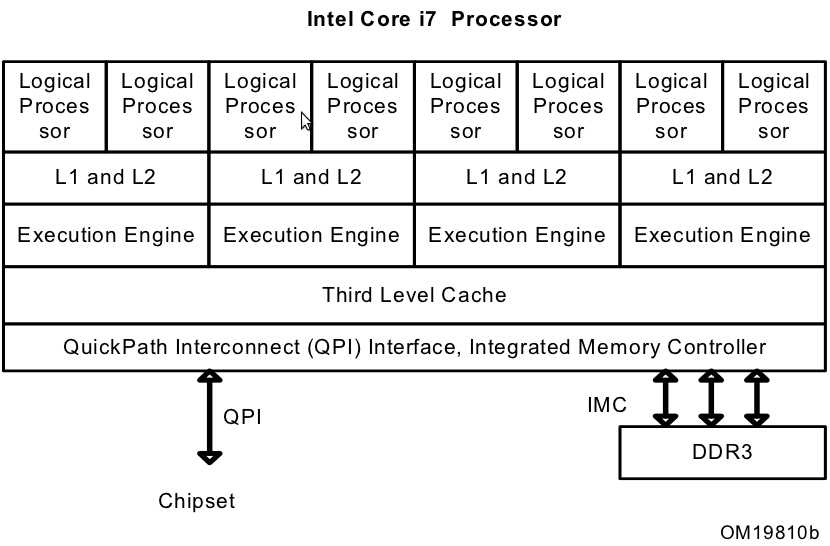
\includegraphics[width=\textwidth]{fig/intel-cache-orga.png}
  \caption{\JWPcpu cache organization (taken from \cite{intel2011softdev})}
  \label{fig:cache-orga}
\end{figure}


\JWlthree{General}

\begin{itemize}

\item organization: see \ref{fig:cache-orga}

\item L1 cache of \SI{64}{\kibi\byte} per core\cite{intel2011softdev}

\item L2 cache of \SI{256}{\kibi\byte} per core\cite{intel2011softdev}

\item shared L3 cache of \SI{8}{\mebi\byte}\cite{intel2011softdev}

\end{itemize}


\JWlthree{PMU}
\label{sec:sandy-bridge-pmu}

\begin{itemize}

\item ca. 184 events available \cite{intel2011events}

\item 8 general-purpose performance counter registers available per core (4 in
      HT mode) \cite{intel2011softdev}

\item 3 fixed performance counter registers (CPU\_CLK\_UNHALTED, INST\_RETIRED,
      ?) \cite{intel2011softdev,intel2011events}

\end{itemize}


\JWlthree{Architectural Differences between Sandy Bridge and Older Architectures}

Cite \cite{fog11}

\begin{itemize}

\item smaller L2 cache but L3 cache

\item branch prediction

\item pipeline changes

\end{itemize}
